\documentclass[12pt,a4paper,titlepage]{article}

\usepackage{preamble}

\title{TP - Analyse subjective-objective de signaux audio}
\author{Yassine Jamoud, Samy Haffoudhi}
\date{\today}

\begin{document}

\maketitle

\section*{Introduction}

Le « bruit de toqué » est obtenu lorsqu’un client « sonne » la planche de bord d’une voiture en frappant dessus avec ses doigts. Il tire de cette information une évaluation subjective de la qualité perçue. L’objectif du TP est de comprendre ce qui fonde, du point de vue du signal, les différences perceptives entre différentes planches, et d’expliquer les préférences utilisateur. Le but ultime de l’étude est de savoir comment reconcevoir la planche de bord (matériaux, montage) pour augmenter la préférence utilisateur.

Nous disposons de 16 sons enregistrés dans des conditions
identiques sur différents véhicules. Ces sons ont été évalués
par un panel d'experts sensoriels selon 5 descripteurs :
\begin{itemize}
    \item{hauteur}
    \item{détonnant}
    \item{attaquant}
    \item{éloignement}
    \item{intensité}
\end{itemize}

\section{Écoute-visualisation des sons}

Nous allons commencer par implémenter une fonction Matlab
permettant de visualiser le signal temporel,
l'analyse spectrale et le spectrogramme d'un son donné.

On obtient par exemple pour le deuxième signal les tracés suivants :

\begin{figure}[H]
  \subfloat[Percentage storage utilization]{
	\begin{minipage}[c][1\width]{
	   0.3\textwidth}
	   \centering
	   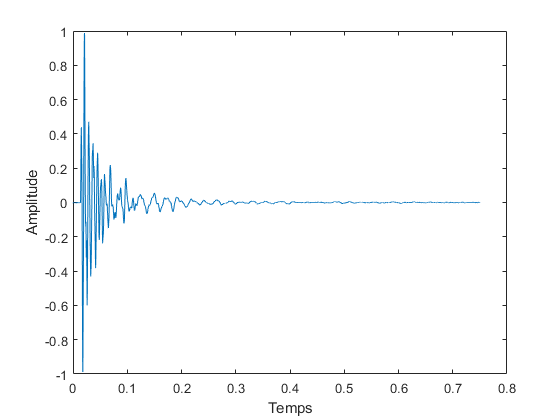
\includegraphics[width=1\textwidth]{temporelle}
	\end{minipage}}
 \hfill
  \subfloat[standard deviation]{
	\begin{minipage}[c][1\width]{
	   0.3\textwidth}
	   \centering
	   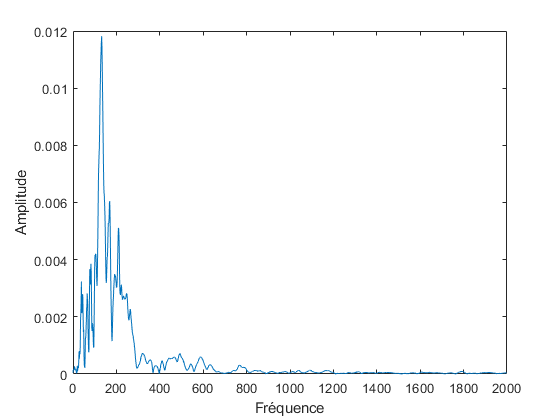
\includegraphics[width=1.1\textwidth]{frequence}
	\end{minipage}}
 hfill
  \subfloat[execution time]{
	\begin{minipage}[c][1\width]{
	   0.3\textwidth}
	   \centering
	   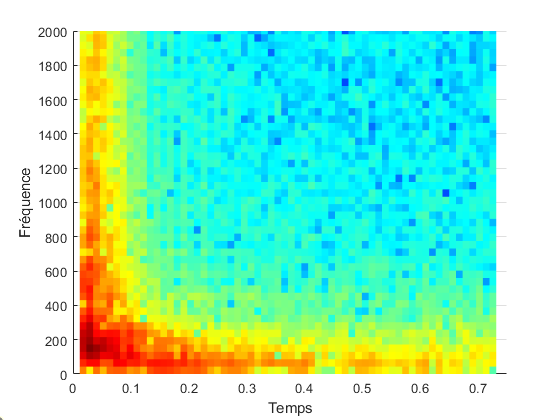
\includegraphics[width=1.2\textwidth]{temps_frequence}
	\end{minipage}}
\caption{}
\end{figure}

On observe alors à partir de ces tracés que :
\begin{itemize}
    \item{L'amplitude du bruit décroit rapidement}
    \item{Le signal contient majoritairement des basses fréquences}
    \item{le contenu fréquenciel devient moins riche au fil du temps}
\end{itemize}

Pour le 18ème son, on obtient :

\begin{figure}[H]
  \subfloat[Percentage storage utilization]{
	\begin{minipage}[c][1\width]{
	   0.3\textwidth}
	   \centering
	   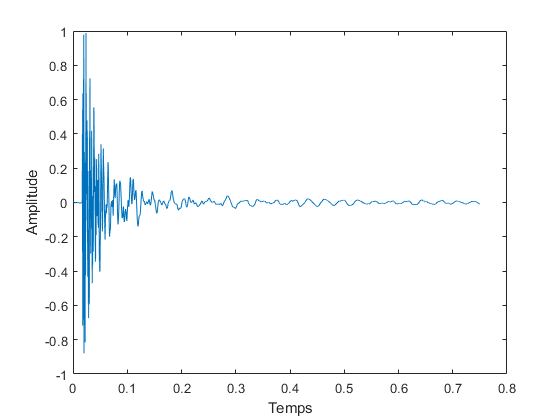
\includegraphics[width=1\textwidth]{temporelle_18}
	\end{minipage}}
 \hfill
  \subfloat[standard deviation]{
	\begin{minipage}[c][1\width]{
	   0.3\textwidth}
	   \centering
	   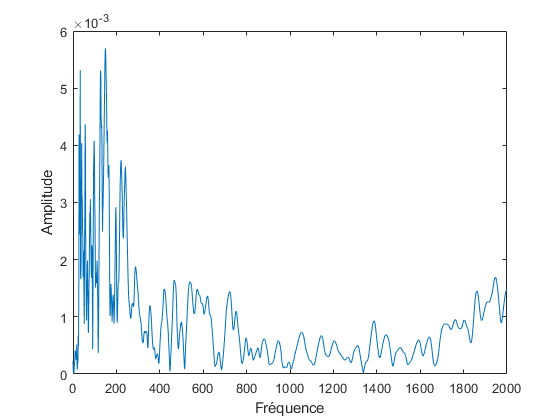
\includegraphics[width=1.1\textwidth]{frequence_18}
	\end{minipage}}
 \hfill
  \subfloat[execution time]{
	\begin{minipage}[c][1\width]{
	   0.3\textwidth}
	   \centering
	   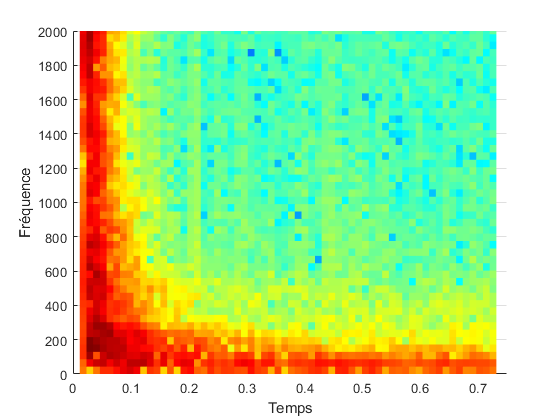
\includegraphics[width=1.2\textwidth]{temps_frequence_18}
	\end{minipage}}
\caption{}
\end{figure}

Cette fois, on observe :
\begin{itemize}
    \item{On ne voit pas de différences marquantes entre les allures temporelles}
    \item{Ce son contient bien plus de hautes fréquences que le son 2}
\end{itemize}

En effet, en écoutant les deux signaux, le son 2 est bien plus agréable
que le son 18.

Par ailleurs, on note l'influence de la taille de la fenêtre sur la précision dans les domaines
fréquentiel et temporel pour le spectrogramme.

\section{Analyse subjective des sons}

Pour une analyse subjective des sons,
on cherche maintenant à effectuer une ACP afin de réaliser:
\begin{itemize}
    \item{L'analyse des composantes principales}
    \item{L'étude des individus}
\end{itemize}

\begin{figure}[H]
    \caption{Cumulative variability}
    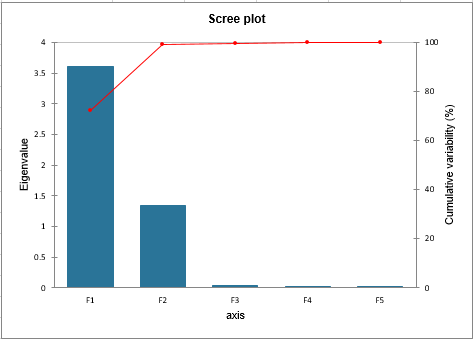
\includegraphics[width=0.5\textwidth]{pca_participation}
    \centering
\end{figure}

On observe ainsi que les deux premiers axes retiennent \textbf{99.114 \%}
d'inertie.

\begin{figure}[H]
    \caption{}
    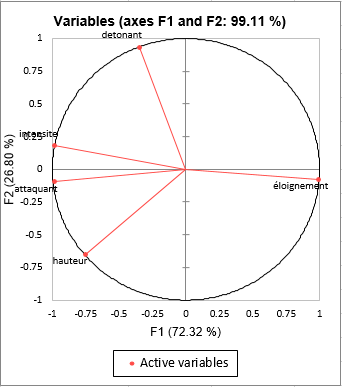
\includegraphics[width=0.3\textwidth]{cercle}
    \centering
\end{figure}

\begin{figure}[H]
    \caption{Squared cosines}
    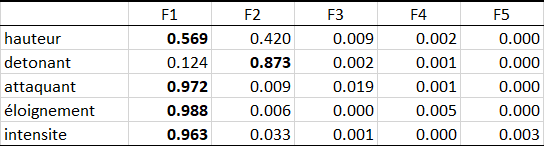
\includegraphics[width=0.5\textwidth]{squared_cosines}
    \centering
\end{figure}

On observe à partir de ces figures que :
\begin{itemize}
    \item{La première composante principale contribue beaucoup à : l'attaquant, l'éloignement et l'intensité}
    \item{La deuxième composante principale contribue beaucoup au détonnant}
    \item{La hauteur repose sur les deux composantes}
\end{itemize}

\begin{figure}[H]
    \caption{biplot}
    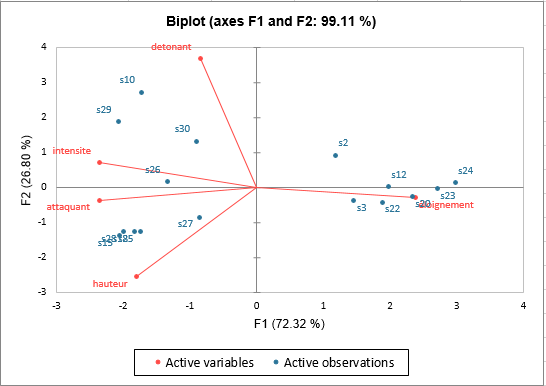
\includegraphics[width=0.7\textwidth]{biplot}
    \centering
\end{figure}

À partir de cette figure, on observe que :
\begin{itemize}
    \item{Un son situé à l'extrémité positive de la CP 1 est caractérisé par un éloignement important}
    \item{Un son situé à l'extrémité négative de la CP 1 est caractérisé par une intensité et un attaquant importants et une hauteur assez importante}
    \item{Un son situé à l'extrémité négative de la CP 2 est caractérisé par une hauteur assez importante}
    \item{Un son situé à l'extrémité positive de la CP 2 est caractérisé par un détonnant important}
    \item{Les sons 2, 12, 24, 3, 22, 20 et 23 contribuent le plus à la CP 1}
    \item{Pour la CP 2, c'est moins homogène}
    \item{Trois clusters seombent se dégager de cette analyse multivariée}
\end{itemize}

Ainsi, on observe que le cluster à droite de la figure est le
plus agréable à l'écoute. Les deux clusters à gauche, sont
globalement assez désagréables même si on observe que le cluster en
haut à gauche reste quand même assez qualitatif.

\section{Analyse objective des sons}

On cherche à extraire différents descripteurs des sons.
On peut ensuite utiliser ces descripteurs pour comparer les
sons entre eux.

Par exemple, pour les sons 2 et 18, on obtient les descripteurs suivants :

\begin{verbatim}
Son 2 :
    lrms: 17.6118
    lmax: 0.9885
    ldb: 57.1380
    kurtosis: 58.6986
    tmax: 0.0180
    tdec: 0.029
    pb: [0.0854 0.5467 0.1293 0.0478 0.0347 0.0288 0.0207 0.0157]
    dba: [7×1 double]
    cdg: 8
    tr1: 0.2604
    tr2: 0.9695
    tr3: 0.0083

Son 18 :
    lrms: 14.6980
    lmax: 0.9885
    ldb: 55.5671
    kurtosis: 39.4787
    tmax: 0.0239
    tdec: 0.052
    pb: [0.1078 0.3457 0.2523 0.2467 0.5667 0.2517 0.2212 0.1761]
    dba: [7×1 double]
    cdg: 8
    tr1: 0.1496
    tr2: 0.3389
    tr3: 0.6449
\end{verbatim}

\section{Étude des corrélations}

On s'intéresse à l'étude des corrélations (corrélation linéaire de Pearson) entre les descripteurs
sensoriel et les descripteurs du signal.

\begin{figure}[H]
    \caption{Matrice de corrélation}
    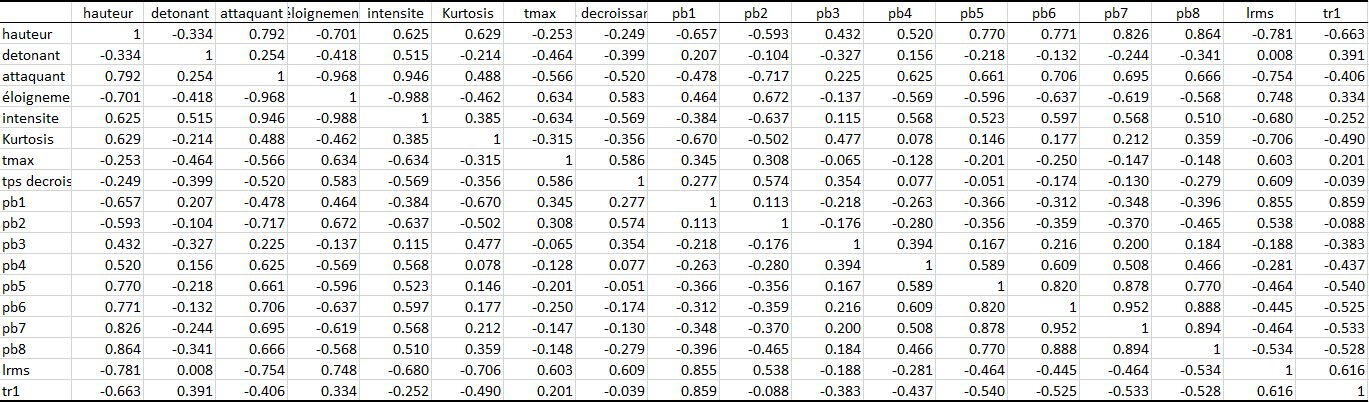
\includegraphics[width=\textwidth]{corr}
    \centering
\end{figure}

On associe à chaque descripteur sensoriel un descripteur du signal qui l'explique :

\begin{itemize}
    \item{Hauteur : pb8}
    \item{Détonnant : $t_max$ coefficient le plus élevé mais quand même assez faible}
    \item{Attaquant : $L_{RMS}$}
    \item{Éloignement : $L_{RMS}$}
    \item{Intensité : $L_{RMS}$}
\end{itemize}

On note en particulier la forte corrélation entre $L_{RMS}$ et les descripteurs sensories différents autre que le détonnant.

\section{Étude de la qualité des sons}

\begin{enumerate}
    \item{On classe les signaux de la façon suivante :
        \begin{verbatim}
Panel	Vous
5.5	    6
4.7	    4
4.5	    4
5.3	    7
2.9	    2
3.4	    3
4.8	    6
5.3	    6
5.7	    7
6.2	    7
3.2	    2
4.3	    4
3.8	    5
3.1	    3
4.6	    5
4.9	    7
    \end{verbatim}
    }

    \item{On projette les cotations de qualité en variables supplémentaires sur le plan de l'ACP des descripteurs sensoriels.
        On obtient la figure suivante :

    \begin{figure}[H]
        \caption{Projection}
        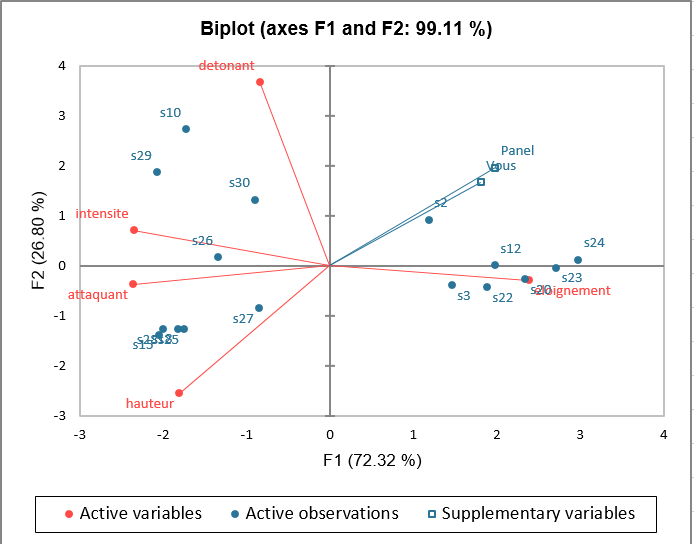
\includegraphics[width=0.7\textwidth]{biplotNous}
        \centering
    \end{figure}

        On obtient alors des résultats cohérents avec notre préférence pour le cluster de droite. On a les même préférences que le pannel.
    }

\item{On représente la cotation de qualité en fonction de chaque décripteur. On obtient les figures suivantes :

    \begin{figure}[H]
        \caption{Intensité}
        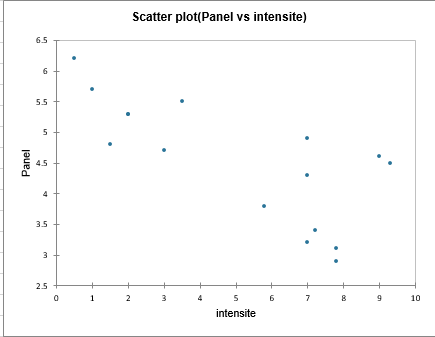
\includegraphics[width=0.5\textwidth]{intensite}
        \centering
    \end{figure}

    \begin{figure}[H]
        \caption{Attaquant}
        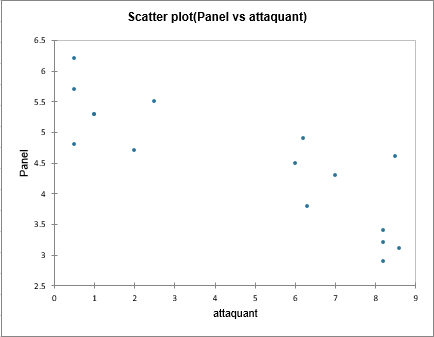
\includegraphics[width=0.5\textwidth]{attaquant}
        \centering
    \end{figure}

    \begin{figure}[H]
        \caption{Détonnant}
        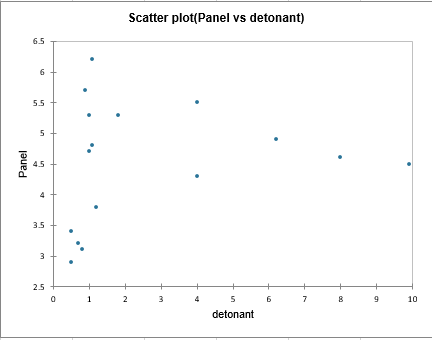
\includegraphics[width=0.5\textwidth]{dettonant}
        \centering
    \end{figure}

    \begin{figure}[H]
        \caption{Éloignement}
        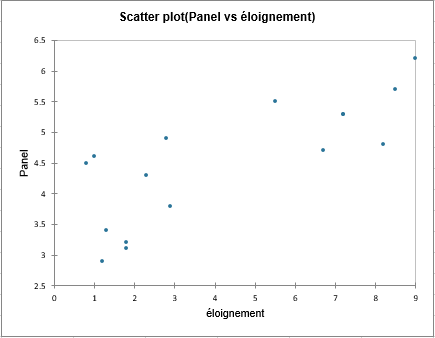
\includegraphics[width=0.5\textwidth]{eloignement}
        \centering
    \end{figure}

    \begin{figure}[H]
        \caption{Hauteur}
        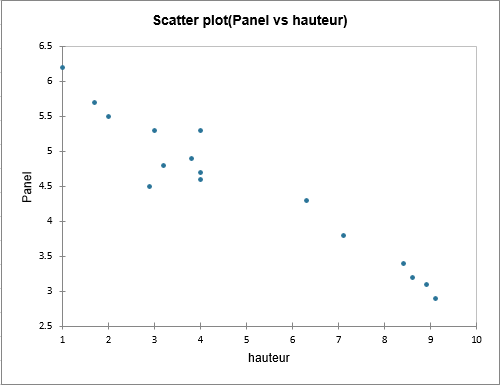
\includegraphics[width=0.5\textwidth]{panel}
        \centering
    \end{figure}

    On obtient la matrice de corrélation suivante :

    \begin{figure}[H]
        \caption{Matrice de corrélation}
        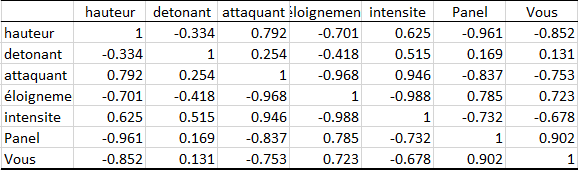
\includegraphics[width=0.7\textwidth]{corr2}
        \centering
    \end{figure}

    On observe alors que les corrélations entre les cotations de qualité et les descripteurs sont très importantes sauf pour le détonnant.

    Enfin, on propose les modèle de régression linéaire suivants :

    \begin{figure}[H]
        \caption{Panel}
        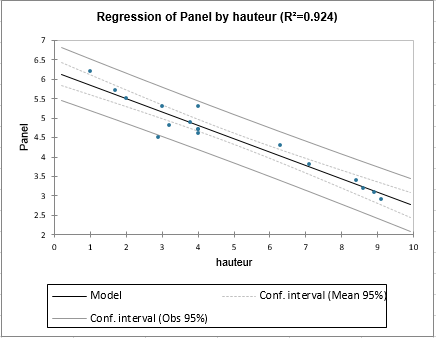
\includegraphics[width=0.5\textwidth]{regression}
        \centering
    \end{figure}

    \begin{figure}[H]
        \caption{Vous}
        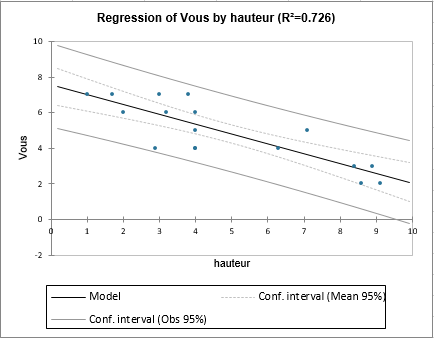
\includegraphics[width=0.5\textwidth]{regression_moi}
        \centering
    \end{figure}

    On obtient $R^2 = 0.924$ pour le cas du panel, une valeur élevée. L'ajustement du modèle est donc correct. La qualité du son décroit donc avec la hauteur.
    La valeur de $R^2$ est moins élevé dans le cas "vous".}

    \item{}

\end{enumerate}

\end{document}
